% Author: PokMan Ho
% Script: res.tex
% Desc: MRes thesis result section
% Input: none
% Output: none
% Arguments: 0
% Date: Jan 2020

\documentclass[../thesis.tex]{subfiles} %% use packages & commands as this main file

\begin{document}
\section{Result}
%% text on all result -> all graphs
%From Table \ref{tab:eqm}, P-only systems (eqm 3) could not give a biologically meaningful result for ``no harvest" setting under the current set of model assumptions.  Hence comparisons between with/without harvest were only done for P+B systems (eqm 4).  Comparing with/without carbon harvest in P+B systems (Fig.\ref{fig:yield}), the effort was statistically higher than ``no harvest" scenario only when the harvest rate was larger than 8/day.  Hence the closest significant sampled harvest rate with ``harvest" $>$ ``no harvest" was 9/day (W=57407, p=0.011).  However out of 1100 samples drew via LHS, about 90\% (n=991, median = -0.0016 (4dp)) feasible scenarios for ``no harvest" setting but only 12\% (n=134, median = 0.5670 (4dp)) for $x=9$/day.  On the other hand, P+B systems with harvest was statistically higher than their P-only counterparts for harvest rates higher than 1/day (Fig.\ref{fig:yield}).  At the closest significant sampled harvest rate with P+B $>$ P-only systems (2/day; W=129849, p$\ll$0.01), all (n=1100, median = -1.1334 (4dp)) scenarios were feasible for P-only system while only 25\% (n=275, median = -0.5379 (4dp)) for the P+B setting.

Addition of bacteria lowered the total carbon content in the system with continuous harvest (Fig.\ref{fig:totC}; $x$ = 0.1/day: W=5914001, p$\ll$0.01, n=3175, Q2\textsubscript{PBH}=1.8620 (4dp), Q2\textsubscript{PoH}=2.5020 (4dp)).  Yet it could be overcome by having higher harvest rate (Fig.\ref{fig:totC}; $x$ = 10/day: W=80556, p$\ll$0.01, n=645, Q2\textsubscript{PBH}=4.1120 (4dp), Q2\textsubscript{PoH}=1.7215 (4dp)).  If considering only the P+B systems, no harvest was always more beneficial in terms of both total carbon (Fig.\ref{fig:totC}, any value of $x$) and yield flux (Fig.\ref{fig:yield}, any value of $x$).  Yield flux was significantly lower in PBH than PoH (Fig.\ref{fig:yield}; $x$ = 10/day: W=406062, p$\ll$0.01, n=645, Q2\textsubscript{PBH}=0.5827 (4dp), Q2\textsubscript{PoH}=1.9074 (4dp))  Destructive harvest (i.e. whole system replacement) recover significantly more carbon than continuous yield (Fig.\ref{fig:yield}, any value of $x$) under the same combinations of biological features.

Effect of biological parameters on the model system (Eq.\ref{eq:ode}) was similar across different harvest rates, hence $x=10$/day was selected for further discussion.  Log total carbon stored in the system for P+B was always higher than that of P-only (Fig.\ref{fig:v2}).  Within the parameter ranges, low phytoplankton growth rate (min feasible $\gP$ = 0.3472/day (4dp)) and high non-respired carbon fraction for bacterial decomposer (max feasible $\eBR$ = 0.9129 (4dp)) could crash the respective systems.  Hence no such high efficient bacteria could be considered; only a P-only scenario could be applied for low growth rate phytoplanktons.  Within feasible parameter ranges, biological parameters affect their systems differently (Fig.\ref{fig:v2}).  Generally speaking, $\ePR$, $\eP$, $\gP$ and $\mB$ had different degree of positive effect on P+B systems (and P-only systems except $\mB$); $\aP$ had a exponential decreasing effect on both P+B and P-only setting; $\eB$ and $\gB$ had a decreasing effect on P+B systems; $\eBR$ had a decreasing effect on yield but an increase in log total carbon.  Note that biological parameters for bacterial decomposer had no effect on P-only system (eqm 3 from Table \ref{tab:eqm})

\begin{figure}[H]
    \centering
    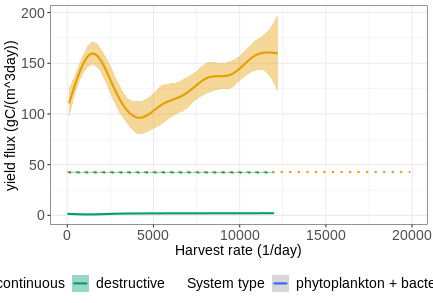
\includegraphics[width=\linewidth]{../result/totC.png}
    \caption[Pairwise log total carbon]{Pairwise log total carbon distribution comparisons of with vs without bacteria and different harvesting scenarios using LHS technique under the temperature range of 23-25\textsuperscript{o}C.  {\scriptsize At each carbon harvest rate (more organic carbon was removed per day on the right, for ``with harvest" systems only), a group of three systems with two Wilcox comparisons were shown.  P+B without harvest (light grey box on the left of each group) was compared (red test annotations at the bottom) with P+B with harvest (orange box on the right of each group) systems.  P-only systems with harvest (green box in the middle of each group) was compared (black test annotations on top) with the right-hand side box in each group.  Each box contained the feasible portion from an original pool of identical sampled 5500 scenarios.  All sample sizes were limited by the fraction of feasible P+B systems with continuous harvest.  Note that the grey boxes in Fig.\ref{fig:yield} are exactly the same as in this figure because the total carbon in systems were equal to the yield under the ``no harvest" setting.}}
    \label{fig:totC}
\end{figure}

\begin{figure}[H]
    \centering
    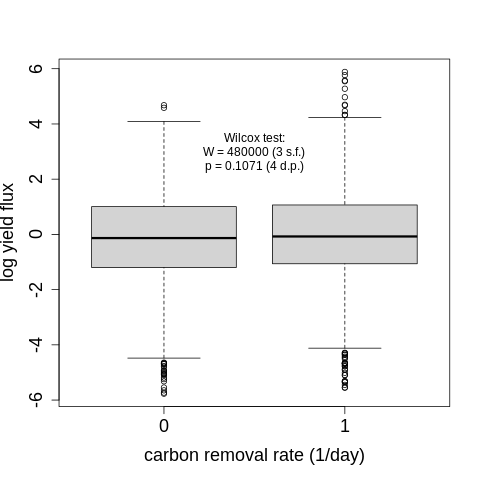
\includegraphics[width=\linewidth]{../result/yield.png}
    \caption[Pairwise log yield flux]{Pairwise log yield flux distribution comparisons of with vs without bacteria and different harvesting scenarios using LHS technique under the temperature range of 23-25\textsuperscript{o}C.  {\scriptsize At each carbon harvest rate (more organic carbon was removed per day on the right, for ``with harvest" systems only), a group of three systems with two Wilcox comparisons were shown.  P+B without harvest (light grey box on the left of each group) was compared (red test annotations at the bottom) with P+B with harvest (orange box on the right of each group) systems.  P-only systems with harvest (green box in the middle of each group) was compared (black test annotations on top) with the right-hand side box in each group.  Each box contained the feasible portion from an original pool of identical sampled 5500 scenarios.  All sample sizes were limited by the fraction of feasible P+B systems with continuous harvest.  Note that the grey boxes in Fig.\ref{fig:totC} are exactly the same as in this figure because the total carbon in systems were equal to the yield under the ``no harvest" setting.}}
    \label{fig:yield}
\end{figure}

\begin{figure}[H]
    \centering
    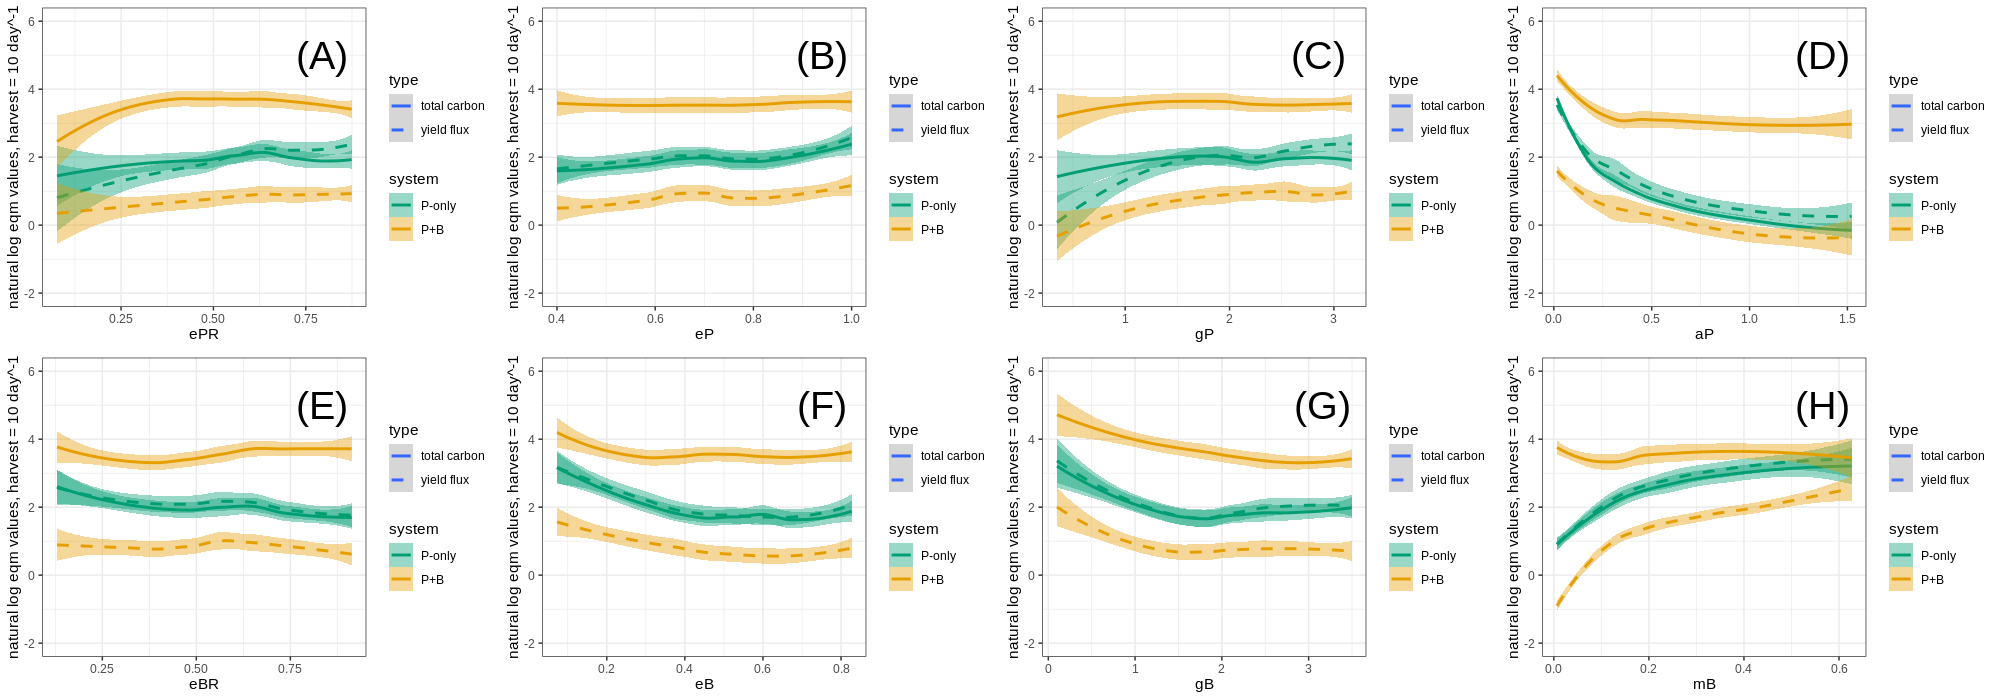
\includegraphics[width=\linewidth]{../result/var_100.png}
    \caption[Log carbon distribution for $x=10day^{-1}$ by parameter]{Distribution for ``log total carbon" (solid line) and ``log yield flux" (dash line) based on respective parameter ranges for P+B (orange) and P-only (green) systems when removal rate = $10day^{-1}$.  {\scriptsize 95\% confidence interval for feasible LHS scenarios across both continuous harvest P+B and P-only systems (N=5500; n=1363) under the temperature range of 23-25\textsuperscript{o}C.  P+B systems were significantly higher than P-only systems in total carbon (W=??, p$\ll$0.01) but lower in yield flux (W=1463831, p$\ll$0.01) under Wilcox signed rank test.}}
    \label{fig:v2}
\end{figure}

\end{document}
